


%----------------------------------
\chapter{Introduction}\label{ch:Planetaryintro}
%----------------------------------

\section{Purpose and Objectives of the \PlanetaryDescT}
%%%%%%%%%%%%%%%%%%%%%%%%%%%%%%%%%%%%%%%%%%%%%%%%%%%%%%%%%%%%%%%%%%%%%%%%%%%%%%%%%
%
% Purpose:  Introduction for the Planetary model.
%
% 
%
%%%%%%%%%%%%%%%%%%%%%%%%%%%%%%%%%%%%%%%%%%%%%%%%%%%%%%%%%%%%%%%%%%%%%%%%%%%%%%%%


%\section{Purpose and Objectives of \PlanetaryDesc}
% Incorporate the intro paragraph that used to begin this Chapter here. 
% This is location of the true introduction where you explain what this model 
% does.
\label{ch:planetaryintro}
The \PlanetaryDesc\ provides the state of a vehicle in three different representations:
\begin{itemize}
\item{Cartesian coordinates}\ \newline
 Cartesian coordinates are centered and fixed with the planet
\item{Spherical coordinates}\ \newline
These are centered on the planet, with $\phi$ measured from the Cartesian z-axis, and $\theta$ measured in the Cartesian x-y plane from the Cartesian x-axis toward the Cartesian y-axis.  The position is represented as \textit{latitude} ($\frac{\pi}{2} - \phi$), \textit{longitude} ($\theta$), and \textit{altitude} ($r - r_{equatorial}$).
\item{Elliptical coordinates}\ \newline
These are also centered on the planet, with elliptical longitude and latitude being measured to the point on the reference ellipsoid (surface) that has a normal that passes through the point of interest.  See Figure~\ref{fig:planetaryellipticalspherical} for a graphical distinction between spherical and elliptical coordinates.
\end{itemize}

\begin{figure}[htp]
\begin{center}
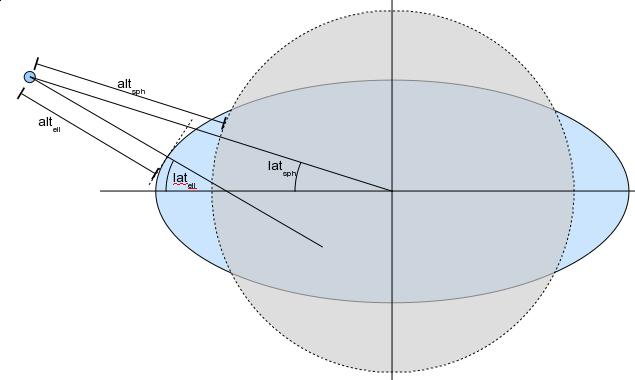
\includegraphics[width=5in]{figures/sphericalelliptical.jpg}
\caption{The differences between spherical and elliptical altitude and latitude.}
\label{fig:planetaryellipticalspherical}
\end{center}
\end{figure}
















%----------------------------------
\chapter{Product Requirements}\label{ch:Planetaryreqt}
%----------------------------------


%%%%%%%%%%%%%%%%%%%%%%%%%%%%%%%%%%%%%%%%%%%%%%%%%%%%%%%%%%%%%%%%%%%%%%%%%%%%%%%%%
%
% Purpose:  requirements for the Planetary model
%
% 
%
%%%%%%%%%%%%%%%%%%%%%%%%%%%%%%%%%%%%%%%%%%%%%%%%%%%%%%%%%%%%%%%%%%%%%%%%%%%%%%%%

% add text here to describe general model requirements
% text is of the form:
\requirement{Planetary representation}
\label{reqt:Planetary}
\begin{description}
  \item[Requirement:]\ \newline
     The Planetary Derived State will provide the capability for expressing the state of one body in a planetary reference frame.
  \item[Rationale:]\ \newline
     Capability from JEOD 1.5.
  \item[Verification:]\ \newline
     Test
\end{description}

\section{Requirements Traceability}

\begin{longtable}[c]{||p{3.5in}|p{3.5in}|}
\caption{Requirements Traceability} \\[6pt]
\hline
{\bf Requirement} & {\bf Inspection and Testing} \\ 
\hline \hline
\endhead
\ref{reqt:Planetary} - Planetary representation &
  Test~\ref{test:Planetary} \\ \hline


\end{longtable}




%----------------------------------
\chapter{Product Specification}\label{ch:Planetaryspec}
%----------------------------------

\section{Conceptual Design}
%%%%%%%%%%%%%%%%%%%%%%%%%%%%%%%%%%%%%%%%%%%%%%%%%%%%%%%%%%%%%%%%%%%%%%%%%%%%%%%%%
%
% Purpose:  Conceptual part of Product Spec for the Planetary model
%
% 
%
%%%%%%%%%%%%%%%%%%%%%%%%%%%%%%%%%%%%%%%%%%%%%%%%%%%%%%%%%%%%%%%%%%%%%%%%%%%%%%%%


%\section{Conceptual Design}

The \PlanetaryDesc\ is used to express the state of a vehicle with respect to a planet-fixed, rotating reference frame.  This is useful, for example, for finding the position of a vehicle with respect to some fixed point on a planetary surface, or for plotting a vehicle trajectory over a map of a planet.

There are three methods for presenting the state, these are described in the \textref{Introduction}{ch:planetaryintro}.
%\section{Mathematical Formulations}
%%%%%%%%%%%%%%%%%%%%%%%%%%%%%%%%%%%%%%%%%%%%%%%%%%%%%%%%%%%%%%%%%%%%%%%%%%%%%%%%%
%
% Purpose:  Mathematical Formulation part of Product Spec for the Planetary model
%
% 
%
%%%%%%%%%%%%%%%%%%%%%%%%%%%%%%%%%%%%%%%%%%%%%%%%%%%%%%%%%%%%%%%%%%%%%%%%%%%%%%%%

\section{Mathematical Formulations}
The mathematical details of the \PlanetaryDesc\ are all handled by other models.  See the Detailed Specification for links.
%\section{Detailed Design}

%%%%%%%%%%%%%%%%%%%%%%%%%%%%%%%%%%%%%%%%%%%%%%%%%%%%%%%%%%%%%%%%%%%%%%%%%%%%%%%%%
%
% Purpose:  Detailed part of Product Spec for the Planetary model
%
% 
%
%%%%%%%%%%%%%%%%%%%%%%%%%%%%%%%%%%%%%%%%%%%%%%%%%%%%%%%%%%%%%%%%%%%%%%%%%%%%%%%%

\section{Detailed Design}
See the \href{file:refman.pdf}{Reference Manual}\cite{derivedstatebib:ReferenceManual} for a summary of member data and member methods for all classes.  

\subsection{Process Architecture}
The architecture for the \PlanetaryDesc\ is trivial, comprising methods that are operationally independent.

\subsection{Functional Design}
This section describes the functional operation of the methods in each class.

The \PlanetaryDesc\ contains only one class:
\begin{itemize}
\classitem{PlanetaryDerivedState}
\textref{DerivedState}{ref:DerivedState}

This contains only the methods \textit{set\_use\_alt\_pfix}, \textit{initialize}, and \textit{update}:
\begin{enumerate}
\funcitem{set\_use\_alt\_pfix}
This method sets the flag indicating whether to use the default planet-centered, planet-fixed reference frame associated with the planet or the alternate one, if one is available for the planet.

\funcitem{initialize}
The initialization process comprises the following steps:
\begin{enumerate}
\item{} The generic DerivedState initialization routine is called to establish the naming convention of the reference object (i.e., the planet about which the vehicle is orbiting) and state identifier.
\item{} The DerivedState method \textit{find\_planet} is called (which subsequently calls the  \href{file:\JEODHOME/models/dynamics/dyn_manager/docs/dyn_manager.pdf}{\em Dynamics Manager}~\cite{dynenv:DYNMANAGER}) method of the same name to find a planet by name; that name is stored as \textit{reference\_name}, and is usually assigned in an input file.
\item{} Depending on the value of \textit{use\_alt\_pfix}, the element \textit{pfix\_ptr} is set to either the default planet-fixed reference frame or the alternate planet-fixed reference frame of the planet identified by \textit{reference\_name} and the frame is subscribed.
\item{} The identified planet is then passed into the initialize method for the PlanetFixedPosition object, \textit{state}, which simply records a pointer to the planet just found in the PlanetFixedPosition class (see \href{file:\JEODHOME/models/utils/planet\_fixed/docs/planet\_fixed.pdf}{\em Planet Fixed} documentation~\cite{dynenv:PLANETFIXED}).
\end{enumerate}

\funcitem{update}
This method uses the RefFrame method \textit{compute\_position\_from} (see \href{file:\JEODHOME/models/utils/ref\_frames/docs/ref\_frames.pdf}{\em Reference Frames} documentation~\cite{dynenv:REFFRAMES}) to calculate the Cartesian position of the \textit{subject} in the planet fixed reference frame.  Then, it uses the PlanetFixedPosition method \textit{update\_from\_cart} 
(see \href{file:\JEODHOME/models/utils/planet\_fixed/docs/planet\_fixed.pdf}{\em Planet Fixed} documentation~\cite{dynenv:PLANETFIXED}) 
to convert the Cartesian representation into spherical and elliptical representations.

\end{enumerate}
\end{itemize}



\chapter{User's Guide}\label{ch:Planetaryuser}
%----------------------------------
The Analysis section of the User's Guide is intended primarily for
users of pre-existing simulations.  
It contains: 
\begin{itemize}
\item A description of how to modify \PlanetaryDesc\ variables after
the simulation
has compiled, including an in-depth discussion of the input file,
\item An overview of how to interpret (but not edit) the S\_define
file,
\item A sample of some of the typical variables that may be logged.
\end{itemize}

The Integration section of the User's Guide is intended for simulation
developers.
It describes the necessary configuration of the \PlanetaryDesc\
within an
S\_define file, and the creation of standard run directories.  The
latter
component assumes a thorough understanding of the preceding Analysis
section of the user guide.
Where applicable, the user may be directed to selected portions of
Product Specification (Chapter \ref{ch:Planetaryspec}).

The Extension section of the User's Guide is intended primarily for
developers
needing to extend the capability of the \PlanetaryDesc.  Such users
should have a
thorough understanding of how the model is used in the preceding
Integration section, and of the model
specification (described in Chapter \ref{ch:Planetaryspec}).


\section{Analysis}
%%%%%%%%%%%%%%%%%%%%%%%%%%%%%%%%%%%%%%%%%%%%%%%%%%%%%%%%%%%%%%%%%%%%%%%%%%%%%%%%%
%
% Purpose:  Analysis part of User's Guide for the Planetary model
%
% 
%
%%%%%%%%%%%%%%%%%%%%%%%%%%%%%%%%%%%%%%%%%%%%%%%%%%%%%%%%%%%%%%%%%%%%%%%%%%%%%%%%

% \section{Analysis}

\label{sec:planetaryuseranalysis}

\subsection{Identifying the \PlanetaryDescT}
If Planet-based states have been included in the simulation, there will be an instance of \textit{PlanetaryDerivedState} located in the S\_define file.  This would typically be found in either the vehicle object, or a separate relative-state object.  There should be an accompanying call to an initialization routine, which takes a reference to the \textit{subject\_body} as one if its inputs, and an accompanying call to an update function.  The \textit{reference\_name} is defined elsewhere, possibly in the input file; this is the name of the planet,with respect to which the state will be evaluated.

Example:
\begin{verbatim}
sim_object{
dynamics/derived_state:    PlanetaryDerivedState example_of_planetary_state;

(initialization) dynamics/derived_state:
example_of_rel_state_object.example_of_planetary_state.initialize (
    Inout DynBody &      subject_body = vehicle_1.dyn_body,
    Inout DynManager &   dyn_manager  = manager_object.dyn_manager);
    
{environment} dynamics/derived_state:
example_of_rel_state_object.example_of_planetary_state.update ( )

} example_of_rel_state_object;
\end{verbatim}

Then the input file may have an entry comparable to:
\begin{verbatim}
example_of_rel_state_object.example_of_planetary_state.reference_name = "Earth";
\end{verbatim}

\subsection{Editing the \PlanetaryDescT}
There is very little to edit in the \PlanetaryDesc, apart from the \textit{reference\_name}, which will result in the planetary state being calculated with respect to a different planet.  It should be noted that \textit{reference\_frame} is only used at initialization, and therefore changing this name \textit{after} the initialization will have no effect.  The \textit{reference\_name} is used to identify the appropriate planet memory location during initialization and thereafter the variable \textit{planet} is used, not \textit{reference\_frame}.

\subsection{Output Data}
The output available from this model is the position of the vehicle with respect to the planet, in planet-fixed coordinates.  This position is available as a Cartesian, spherical, or elliptical coordinate representation.
\begin{verbatim}
example_of_rel_state_object.example_of_planetary_state.state.cart_coords[0-2]
example_of_rel_state_object.example_of_planetary_state.state.sphere_coords.altitude
example_of_rel_state_object.example_of_planetary_state.state.sphere_coords.latitude
example_of_rel_state_object.example_of_planetary_state.state.sphere_coords.longitude
example_of_rel_state_object.example_of_planetary_state.state.ellip_coords.altitude
example_of_rel_state_object.example_of_planetary_state.state.ellip_coords.latitude
example_of_rel_state_object.example_of_planetary_state.state.ellip_coords.longitude
\end{verbatim}

The rotational state is not available.

%\section{Integration}
%%%%%%%%%%%%%%%%%%%%%%%%%%%%%%%%%%%%%%%%%%%%%%%%%%%%%%%%%%%%%%%%%%%%%%%%%%%%%%%%%
%
% Purpose:  Integration part of User's Guide for the Planetary model
%
% 
%
%%%%%%%%%%%%%%%%%%%%%%%%%%%%%%%%%%%%%%%%%%%%%%%%%%%%%%%%%%%%%%%%%%%%%%%%%%%%%%%%

 \section{Integration}

Including the \PlanetaryDesc\ is relatively straightforward.

 \subsection{Generating the S\_define}

Conventional practice would add the \PlanetaryDesc\ to the vehicle object, or (if one exists) to a separate relative-state object at the end of the S\_define file.  When adding the state to a specific vehicle, care must be taken to ensure that the calls to update the state occur after the planet position has been generated from the ephemerides, and the vehicle position integrated.  There is no internal check that this ordering is achieved, the responsibility for ensuring this lies entirely on the Integrator.

The instance of \textit{PlanetaryDerivedState} needs to be defined, the model initialized, and a routine update scheduled.  A simple example of how this may look is found in the \textref{Analysis}{sec:planetaryuseranalysis} section.  Simple example simulations are found in the 
\textit{derived\_state/verif/Planetary} verification simulations released with \JEODid.

\subsection{Generating the Input File}
The input file (or Modified Data file) must contain the name of the planet, identified as \textit{reference\_name}.

In the input file, the user may specify which planet-centered, planet-fixed reference frame (default or alternate) to use as the basis of the position calculations. Note: this only works with Planets that have an alternate reference frame defined.
\begin{verbatim}
example_of_rel_state_object.example_of_planetary_state.set_use_alt_pfix(False);

\end{verbatim}
or
\begin{verbatim}
example_of_rel_state_object.example_of_planetary_state.set_use_alt_pfix(True);

\end{verbatim}

See the \textref{Analysis}{sec:planetaryuseranalysis} section for an example of how the input data may appear.

\subsection{Logging the Data}
See the \textref{Analysis}{sec:planetaryuseranalysis} section for a list of available output data.


%\section{Extension}
%%%%%%%%%%%%%%%%%%%%%%%%%%%%%%%%%%%%%%%%%%%%%%%%%%%%%%%%%%%%%%%%%%%%%%%%%%%%%%%%%
%
% Purpose:  Extension part of User's Guide for the Planetary model
%
% 
%
%%%%%%%%%%%%%%%%%%%%%%%%%%%%%%%%%%%%%%%%%%%%%%%%%%%%%%%%%%%%%%%%%%%%%%%%%%%%%%%%

 \section{Extension}

The \PlanetaryDesc\ is not intended to be extensible.

%----------------------------------
\chapter{Verification and
Validation}\label{ch:Planetaryivv}
%----------------------------------

\section{Verification}
%%%%%%%%%%%%%%%%%%%%%%%%%%%%%%%%%%%%%%%%%%%%%%%%%%%%%%%%%%%%%%%%%%%%%%%%%%%%%%%%%
%
% Purpose:  Verification part of V&V for the Planetary model
%
% 
%
%%%%%%%%%%%%%%%%%%%%%%%%%%%%%%%%%%%%%%%%%%%%%%%%%%%%%%%%%%%%%%%%%%%%%%%%%%%%%%%%

% \section{Verification}

%%% code imported from old template structure
\label{ch:planetaryvv}

\subsection{Inspection of Modeling Requirements}

\inspection{State Encapsulation}\label{inspect:Planetary}
 The \PlanetaryDesc\ is capable of outputting data as desired, thereby satisfying
 requirement \ref{reqt:Planetary} at the inspection level.  The validity of the output data is tested below.


\subsection{Verification of Surface Representations}

\test{Verification of \PlanetaryDesc\ Output Data for Generic Orbits}\label{test:Planetary}

\begin{description}
\item{Purpose:}\newline
To demonstrate that the data output by the \PlanetaryDesc\ provides meaningful data.

\item{Requirements:}\newline
Satisfactory conclusion of this test satisfies requirement \ref{reqt:Planetary}

\item{Procedure:}\newline
A simulation was developed containing an arbitrary vehicle initialized into one of several orbits:
\begin{enumerate}
 \item {Low Earth Orbit, equatorial.}\ \newline  
Initialized with an apo-altitude and peri-altitude of 400 km, and an inclination of zero.
 \item {Low Earth Orbit, inclined.}  \ \newline
Initialized with an apo-altitude and peri-altitude of 400 km, and an inclination of 45 degrees.
 \item {Low Earth Orbit, polar.}\ \newline
  Initialized with an apo-altitude and peri-altitude of 400 km, and an inclination of 90 degrees.
 \item {Eccentric Earth Orbit, equatorial.}\ \newline
  Initialized with an apo-altitude of 8,000 km, a peri-altitude of 400 km, and an inclination of zero.
 \item {Near-Geosynchronous Orbit.}\ \newline
  Initialized with an apo-altitude and peri-altitude of 35,786 km, and an inclination of zero.
\end{enumerate}
The data from the five simulations were compared against theory and against each other. 


\item{Predictions:}
\begin{enumerate}
 \item {Low Earth Orbit, equatorial}
\begin{itemize}
\item{}The Cartesian coordinate output from this data should be close to 0 on the z-axis, and be oscillatory on the x-and y- axes, with a period equal to the synodic period of the satellite, approximately 5,940 seconds.
\item{}The inertial position should oscillate on all three axes with a period equal to the sidereal period of the satellite, approximately 5,560 seconds.
\item{}The altitude should remain approximately constant. The longitude should have a saw-tooth appearance with a variation that is linear with time, rising to $\pi$ radians, and resetting to $-\pi$ radians instantaneously, with a period equal to the synodic period of the satellite. The latitude should remain at zero.
\end{itemize}

\item {Low Earth Orbit, inclined}
\begin{itemize}
\item{}The Cartesian coordinate output from this data should show the same periodic behavior as for the equatorial orbit on the x- and y-axes, with an additional 1-day oscillation in the magnitude of the x- and y- axis magnitudes due to the rotation of Earth underneath the orbit (when the orbital nodes lie close to the x-axis, the x-axis oscillation should be close to the full magnitude of 6,800 km, and the y-axis oscillation only at $6,778 km ~ \sin (\pi / 2) =  4,800 km$, and vice-versa.
On the z-axis, there should be some oscillation with a magnitude of approximately $6,778 km ~ \sin (\pi / 2) =  4,800 km$, and a period equal to the sidereal period of approximately 5,560 seconds.
\item{}The inertial position should show a similar pattern to that for the equatorial orbit, with the same period.
\item{}The altitude should remain approximately constant when expressed in spherical coordinates, but differ significantly when expressed in elliptical (geodetic) coordinates to account for the reduced radius of Earth at higher latitudes.  The difference between the elliptical altitude and spherical altitude should be maximized at high latitudes, and zero at equatorial latitudes.  The period of this oscillation should be the sidereal period of the satellite.
The longitude should exhibit a saw-tooth pattern, but the rise is not expected to be linear; the vehicle will be covering longitude more rapidly at high latitudes than near the equator; while its speed is constant, the vehicle is traveling perpendicular to lines of longitude at high latitudes, but not at equatorial latitudes.  The period of this oscillation should be the synodic period of the satellite.
The latitude should oscillate between $\pm \frac{\pi}{4}$ with a period equal to the sidereal period.
\end{itemize}

\item {Low Earth Orbit, polar}
\begin{itemize}
\item{}The Cartesian coordinate output from this data should continue the trend seen in going to a 45 degree inclination; the z-axis amplitude should increase to the full 6,800 km, and the day-long oscillation on the x-and y-axes should force their respective amplitudes to vary between 0 and the full 6,800 km, ninety degrees out of phase with each other.
\item{}The inertial position should should show a similar pattern to that for the equatorial orbit, with the same period.
\item{}The altitude should show the same pattern as exhibited for the inclined orbit, but with the geodetic altitude reaching a maximum of 21 km above the spherical altitude as the vehicle crosses the poles.
The longitude should show a day-long trend, with a transition at every polar crossing of $\pi$ radians.
The latitude should show a linear triangular oscillation as the latitude varies uniformly while the vehicle heading is northerly and southerly at a constant rate.
\end{itemize}

\item {Eccentric Earth Orbit, equatorial}
\begin{itemize}
\item{}The altitude will vary significantly.  Because of the difference in speed between apoapsis and periapsis, this variation will not be sinusoidal, but should have a steeper gradient near periapsis.  The altitude will oscillate with the sidereal period of the vehicle.
The longitude should exhibit a quasi-sawtooth pattern, but will have significant variation in its gradient due to the varying speed and proximity of the vehicle (when the vehicle is closer, at the same speed, it should cover more longitude in any given time step; when the vehicle is closer, it is also moving faster, exacerbating this feature).  The longitude oscillation will be at the synodic period of the vehicle, whereas the proximity of the vehicle to the planet oscillates at the sidereal period.  Therefore, the ``sawteeth'' are not expected to be equal, the section of the tooth with a steep gradient (vehicle is close to the planet) will gradually migrate across the tooth edge. 
The latitude should remain at zero.  The altitude should oscillate non-sinusoidally, but with constant amplitude on each axis since the orbit is not rotating with respect to the inertial axes (orbital precession is neglected since the orbit is so close to equatorial) 
\item{}The Cartesian coordinate output from this data should exhibit oscillatory-on-oscillatory behavior, as the x- and y-axes rotate on and off the major axis of the orbit.  The oscillation should not be sinusoidal, as observed for the altitude-longitude-latitude plot.
\item{}The inertial position should exhibit non-sinusoidal oscillatory behavior on all three axes, with each axis having constant amplitude over time.  The three axes must not be in phase, and there is no expectation on the relative magnitude of the oscillation from axis to axis.
\end{itemize}

\item {Near-Geosynchronous Orbit.}
\begin{itemize}
\item{}The Cartesian coordinate output from this data should show minimal variation on all three axes; the vehicle should be stationary above a constant point on Earth.
\item{}The inertial position should show one complete oscillation (simulation ran for 24 hours) on all three axes.
\item{}The altitude, latitude, and longitude should all show minimal variation through the simulation.
\end{itemize}

\end{enumerate}

\item{Results:}
\begin{enumerate}
 \item {Low Earth Orbit, equatorial.}
\begin{itemize}
\item{}The Cartesian coordinate gradually diverge from 0 on the z-axis, but by less than 10 meters over a day.  The period of oscillation on the other axes matches that from prediction.  See Figure~\ref{fig:planetaryleoequcart}
\item{}The inertial position oscillates on all three axes with a period equal to that predicted.  See Figure~\ref{fig:planetaryleoequinrtl}
\item{}The altitude remains approximately constant (the variation seen in Figure~\ref{fig:planetaryleoequlal} is less than 1 meter). The longitude exhibits the expected saw-tooth appearance with the correct period. The latitude diverges slowly from zero, but only to less than a micro-radian.  See Figure~\ref{fig:planetaryleoequlal}.
\end{itemize}

\begin{figure}[!ht]
  \begin{center}
        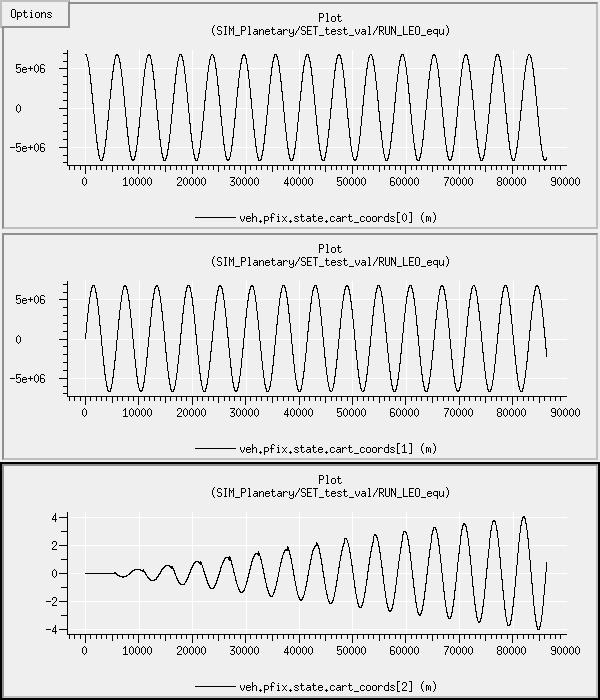
\includegraphics[width=80mm]{figures/planetary_leo_equ_cart.jpg}
        \caption{The variation of position with time, expressed in Cartesian coordinates.} 
        \label{fig:planetaryleoequcart}
  \end{center}
\end{figure}

\begin{figure}[!ht]
  \begin{center}
        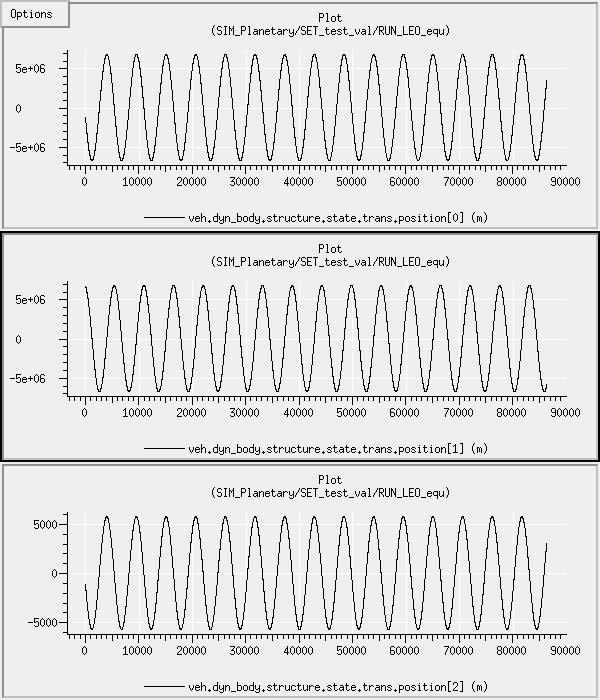
\includegraphics[width=80mm]{figures/planetary_leo_equ_inrtl.jpg}
        \caption{The variation of position with time, expressed in inertial coordinates.} 
        \label{fig:planetaryleoequinrtl}
  \end{center}
\end{figure}

\begin{figure}[!ht]
  \begin{center}
        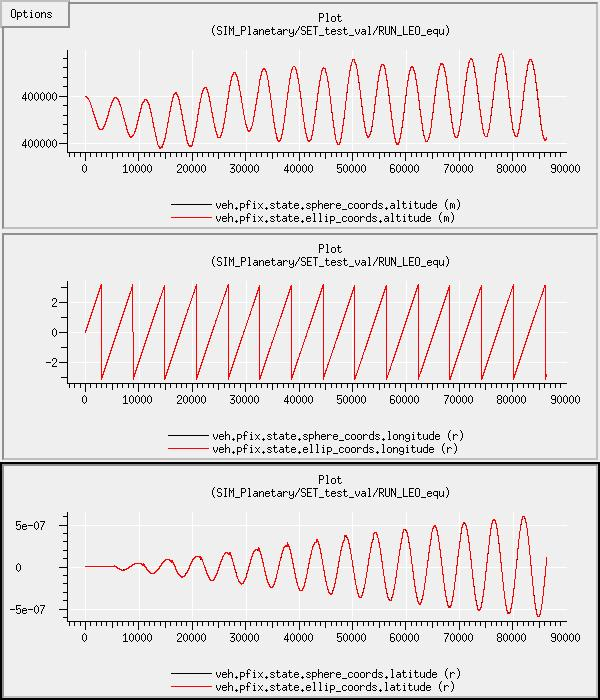
\includegraphics[width=80mm]{figures/planetary_leo_equ_lal.jpg}
        \caption{The variation of position with time, expressed in Altitude-Longitude-Latitude coordinates, both spherical and elliptical (geodetic).} 
        \label{fig:planetaryleoequlal}
  \end{center}
\end{figure}

\clearpage

\item {Low Earth Orbit, inclined.}\ \newline
All data is as expected.  See Figures~\ref{fig:planetaryleoinccart}, \ref{fig:planetaryleoincinrtl}, and~\ref{fig:planetaryleoinclal}.  Figure~\ref{fig:planetaryleoincinrtl} superposes the data from the equatorial low-altitude orbit with that from the inclined low-altitude orbit.

\begin{figure}[!ht]
  \begin{center}
        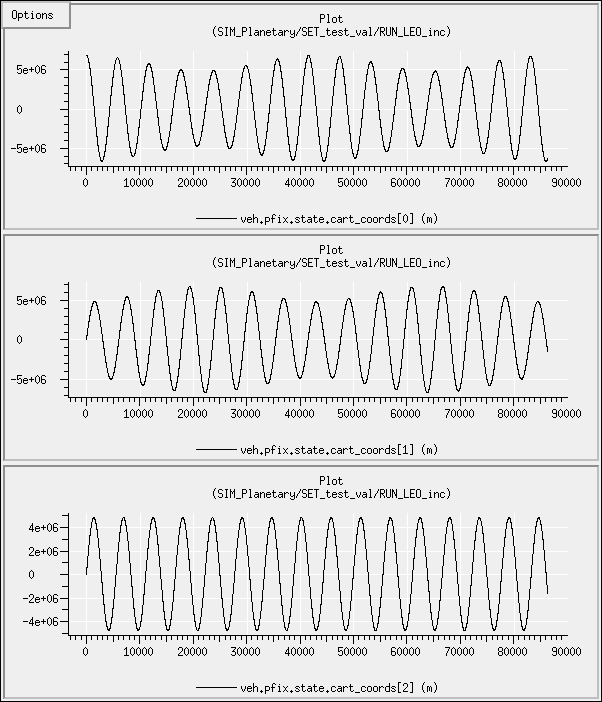
\includegraphics[width=80mm]{figures/planetary_leo_inc_cart.jpg}
        \caption{The variation of position with time, expressed in Cartesian coordinates.} 
        \label{fig:planetaryleoinccart}
  \end{center}
\end{figure}

\begin{figure}[!ht]
  \begin{center}
        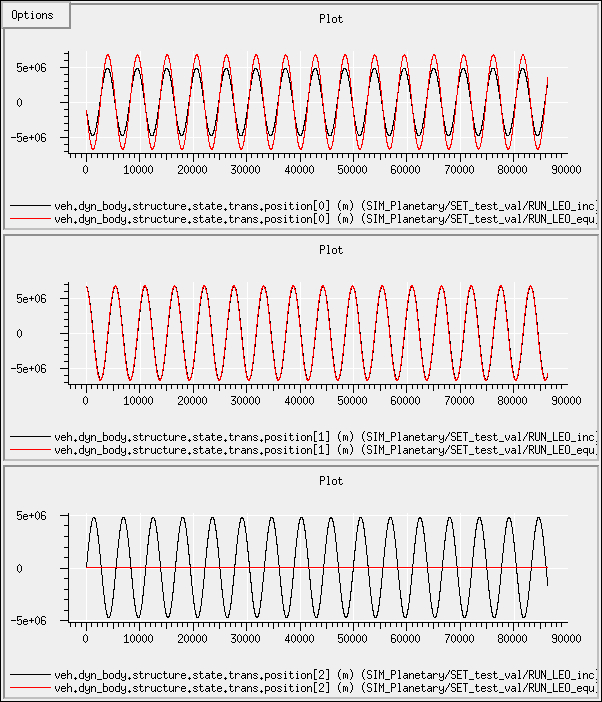
\includegraphics[width=80mm]{figures/planetary_leo_inc_inrtl.jpg}
        \caption{The variation of position with time, expressed in inertial coordinates.} 
        \label{fig:planetaryleoincinrtl}
  \end{center}
\end{figure}

\begin{figure}[!ht]
  \begin{center}
        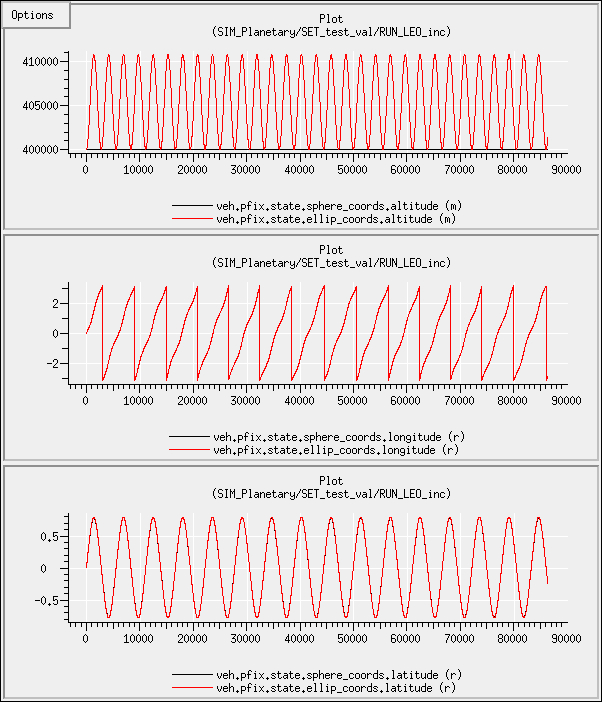
\includegraphics[width=80mm]{figures/planetary_leo_inc_lal.jpg}
        \caption{The variation of position with time, expressed in Altitude-Longitude-Latitude coordinates, both spherical and elliptical (geodetic).} 
        \label{fig:planetaryleoinclal}
  \end{center}
\end{figure}

\clearpage

\item {Low Earth Orbit, polar.}\ \newline
All data is as expected.  See Figures~\ref{fig:planetaryleopolarcart}, \ref{fig:planetaryleopolarinrtl}, and~\ref{fig:planetaryleopolarlal}.  Figure~\ref{fig:planetaryleopolarinrtl} superposes the data from the equatorial low-altitude orbit with that from the inclined low-altitude orbit and the low-altitude polar orbit.

\begin{figure}[!ht]
  \begin{center}
        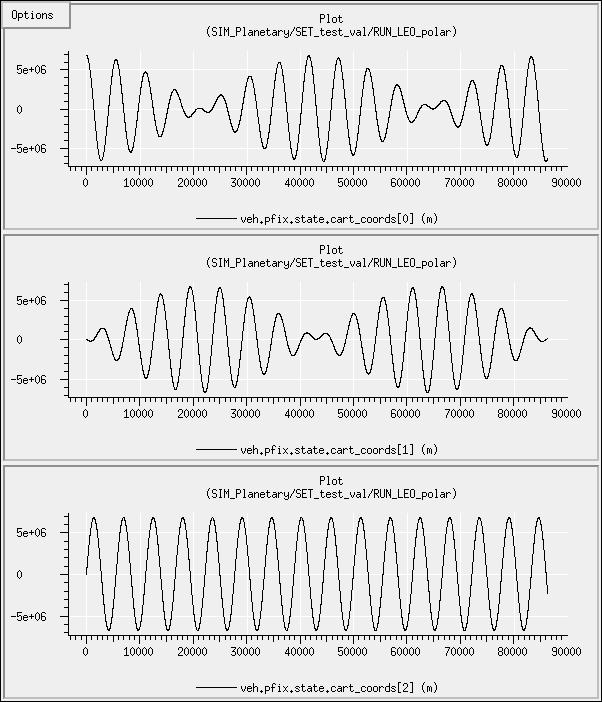
\includegraphics[width=80mm]{figures/planetary_leo_polar_cart.jpg}
        \caption{The variation of position with time, expressed in Cartesian coordinates.} 
        \label{fig:planetaryleopolarcart}
  \end{center}
\end{figure}

\begin{figure}[!ht]
  \begin{center}
        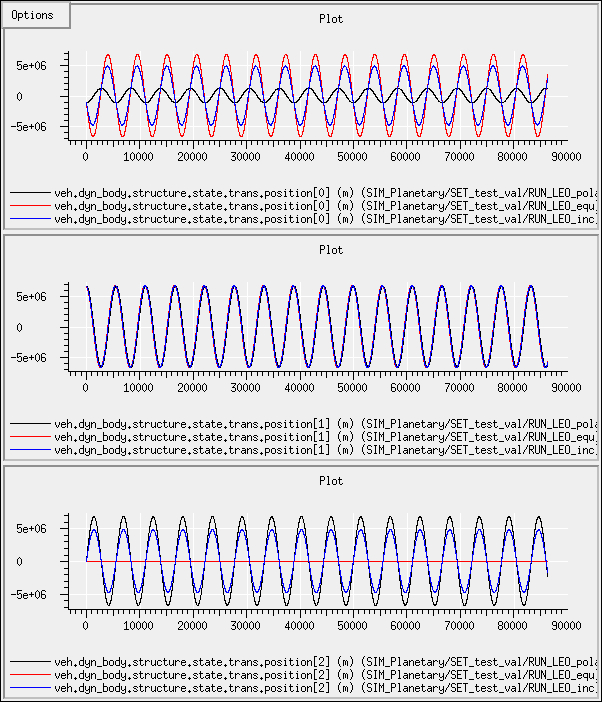
\includegraphics[width=80mm]{figures/planetary_leo_polar_inrtl.jpg}
        \caption{The variation of position with time, expressed in inertial coordinates.} 
        \label{fig:planetaryleopolarinrtl}
  \end{center}
\end{figure}

\begin{figure}[!ht]
  \begin{center}
        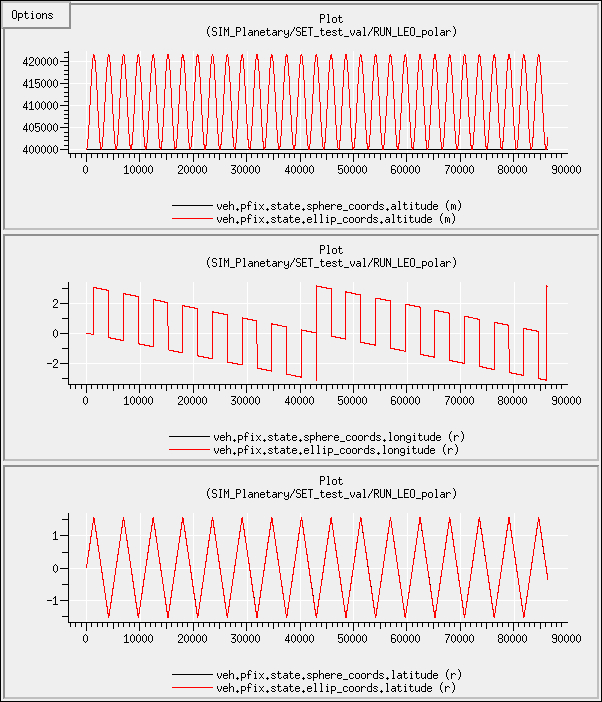
\includegraphics[width=80mm]{figures/planetary_leo_polar_lal.jpg}
        \caption{The variation of position with time, expressed in Altitude-Longitude-Latitude coordinates, both spherical and elliptical (geodetic).} 
        \label{fig:planetaryleopolarlal}
  \end{center}
\end{figure}

\clearpage

\item {Eccentric Earth Orbit, equatorial.}\ \newline
All data is as expected.  See Figures~\ref{fig:planetaryleoecccart}, \ref{fig:planetaryleoeccinrtl}, and~\ref{fig:planetaryleoecclal}.  

\begin{figure}[!ht]
  \begin{center}
        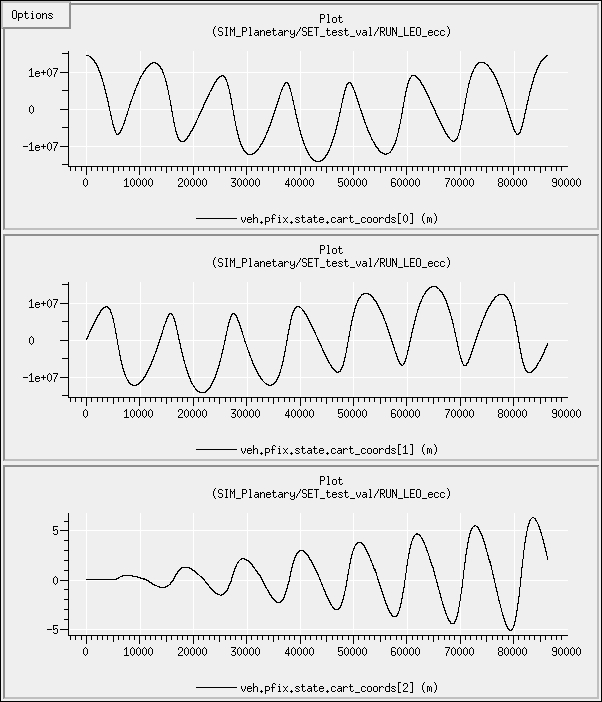
\includegraphics[width=80mm]{figures/planetary_leo_ecc_cart.jpg}
        \caption{The variation of position with time, expressed in Cartesian coordinates.} 
        \label{fig:planetaryleoecccart}
  \end{center}
\end{figure}

\begin{figure}[!ht]
  \begin{center}
        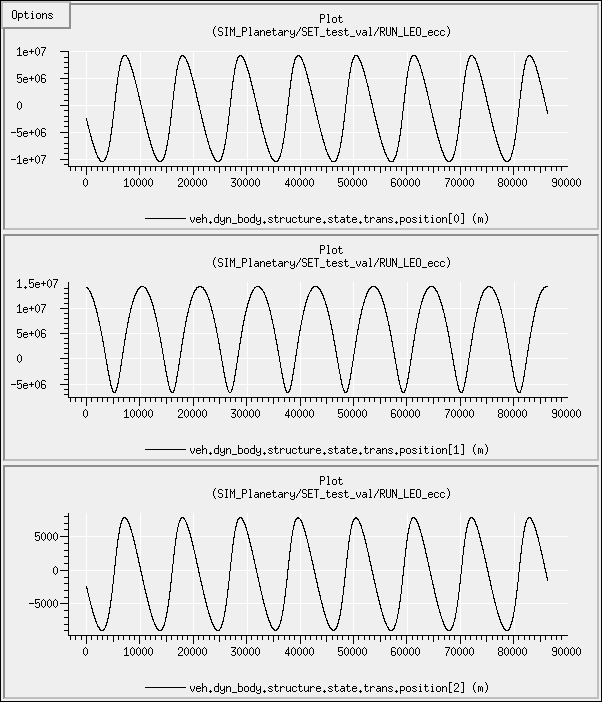
\includegraphics[width=80mm]{figures/planetary_leo_ecc_inrtl.jpg}
        \caption{The variation of position with time, expressed in inertial coordinates.} 
        \label{fig:planetaryleoeccinrtl}
  \end{center}
\end{figure}

\begin{figure}[!ht]
  \begin{center}
        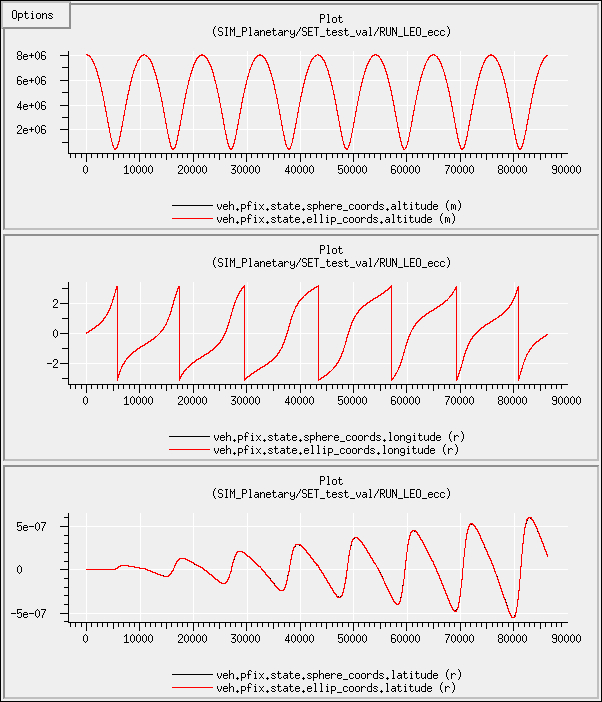
\includegraphics[width=80mm]{figures/planetary_leo_ecc_lal.jpg}
        \caption{The variation of position with time, expressed in Altitude-Longitude-Latitude coordinates, both spherical and elliptical (geodetic).} 
        \label{fig:planetaryleoecclal}
  \end{center}
\end{figure}

\clearpage

\item {Near-Geosynchronous Orbit.}\ \newline
All data is as expected.  See Figures~\ref{fig:planetarygeocart}, \ref{fig:planetarygeoinrtl}, and~\ref{fig:planetarygeolal}.  Note that the variations on the Cartesian and altitude, longitude, latitude values are generally quite small, with the vehicle advancing very slowly along its orbit; this is most likely a result of an altitude that is not quite appropriate for a geosynchronous orbit.
\end{enumerate}

\begin{figure}[!ht]
  \begin{center}
        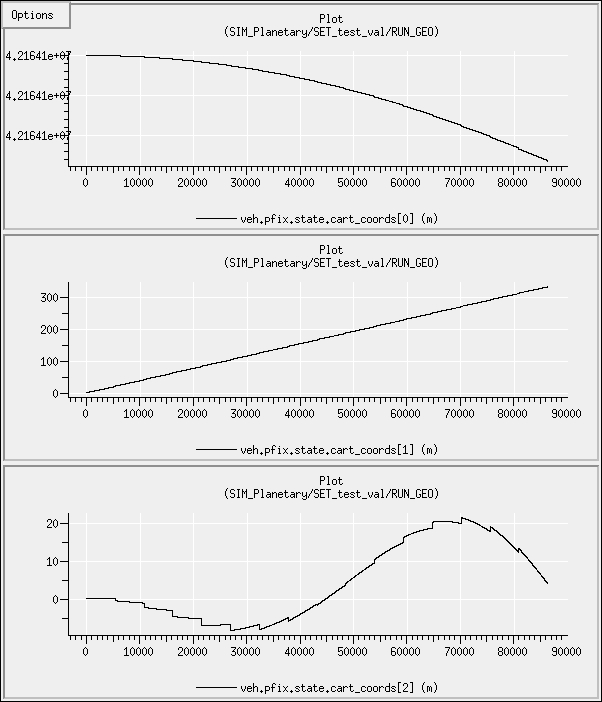
\includegraphics[width=80mm]{figures/planetary_geo_cart.jpg}
        \caption{The variation of position with time, expressed in Cartesian coordinates.} 
        \label{fig:planetarygeocart}
  \end{center}
\end{figure}

\begin{figure}[!ht]
  \begin{center}
        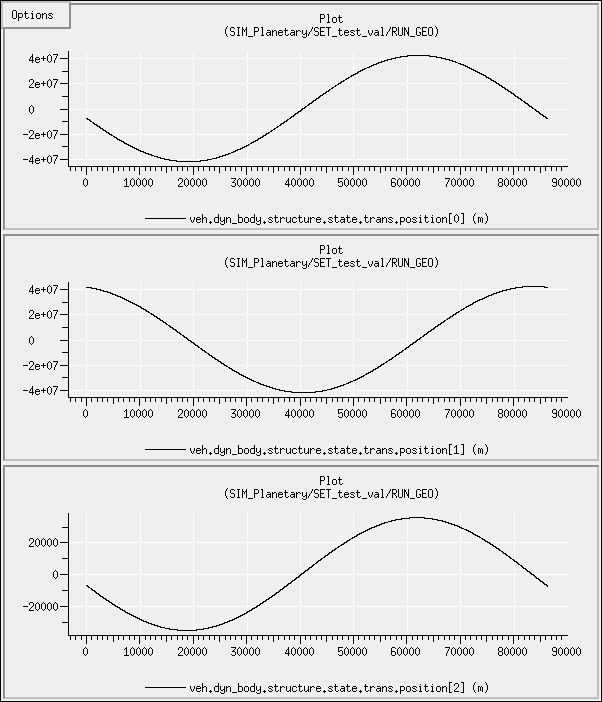
\includegraphics[width=80mm]{figures/planetary_geo_inrtl.jpg}
        \caption{The variation of position with time, expressed in inertial coordinates.} 
        \label{fig:planetarygeoinrtl}
  \end{center}
\end{figure}

\begin{figure}[!ht]
  \begin{center}
        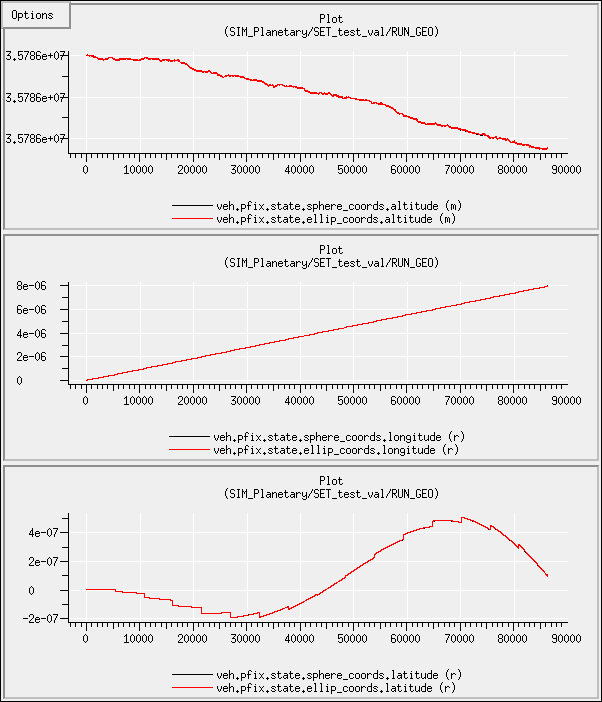
\includegraphics[width=80mm]{figures/planetary_geo_lal.jpg}
        \caption{The variation of position with time, expressed in Altitude-Longitude-Latitude coordinates, both spherical and elliptical (geodetic).} 
        \label{fig:planetarygeolal}
  \end{center}
\end{figure}

\clearpage

\end{description}





%\section{Validation}
%%%%%%%%%%%%%%%%%%%%%%%%%%%%%%%%%%%%%%%%%%%%%%%%%%%%%%%%%%%%%%%%%%%%%%%%%%%%%%%%%
%
% Purpose:  Validation part of V&V for the Planetary model
%
% 
%
%%%%%%%%%%%%%%%%%%%%%%%%%%%%%%%%%%%%%%%%%%%%%%%%%%%%%%%%%%%%%%%%%%%%%%%%%%%%%%%%

\section{Validation}

%%% code imported from old template structure
%\test{<Title>}\label{test:<label>}
%\begin{description}
%\item[Purpose:] \ \newline
%<description>
%\item[Requirements:] \ \newline
%By passing this test, the universal time module 
%partially satisfies requirement~\ref{reqt:<label1>} and 
%completely satisfies requirement~\ref{reqt:<label2>}.
%\item[Procedure:]\ \newline
%<procedure>
%\item[Results:]\ \newline
%<results>
%\end{description}

This method has not been validated against external data.


